\newcounter{choice}
\renewcommand\thechoice{\Alph{choice}}
\newcommand\choicelabel{\thechoice.}

\newenvironment{choices}%
  {\list{\choicelabel}%
     {\usecounter{choice}\def\makelabel##1{\hss\llap{##1}}%
       \settowidth{\leftmargin}{W.\hskip\labelsep\hskip 2.5em}%
       \def\choice{%
         \item
       } % choice
       \labelwidth\leftmargin\advance\labelwidth-\labelsep
       \topsep=0pt
       \partopsep=0pt
     }%
  }%
  {\endlist}

% A
\chapter{การหาค่าความเที่ยงตรงของแบบสอบถาม IOC: Index of item objective congruence} \label{app1}

การหาค่า IOC ของผู้เชี่ยวชาญ จากการให้ผู้เชี่ยวชาญตรวจสอบแบบสอบถามการวิจัย IOC คือค่าความเที่ยงตรงของแบบสอบถามหรือ ค่าสอดคล้อง
ระหว่างข้อคำถามกับวัตถุประสงค์หรือเนื้อหา ปกติแล้วจะให้ผู้เชี่ยวชาญตรวจสอบ ตั้งแต่ 3 คนขึ้นไปในการตรวจสอบ

\section{เกณฑ์การพิจารณาข้อคำถาม}
\begin{enumerate}
    \item ให้คะแนน +1 ถ้าแน่ใจว่าข้อคำถามวัดได้ตรงตามวัตถุประสงค์
    \item ให้คะแนน 0 ถ้าไม่แน่ใจว่าข้อคำถามวัดได้ตรงตามวัตถุประสงค์
    \item ให้คะแนน -1 ถ้าแน่ใจว่าข้อคำถามสัดได้ไม่ตรงตามวัตถุประสงค์
\end{enumerate}

\section{การหาค่า IOC ในแต่ละหัวข้อ}
วิธีหาค่าของ IOC คือการนำคะแนนรวมของผู้เชี่ยวชาญในแต่ละหัวข้อมาหารด้วยจำนวณของผู้เชี่ยวชาญ

\section{เกณฑ์ความเที่ยงตรง}
\begin{enumerate}
    \item ข้อคำถามที่มีค่า IOC ตั้งแต่ 0.50--1.00 มีค่าความเที่ยงตรงที่ใช้ได้
    \item ข้อคำถามที่มีค่า IOC ต่ำกว่า 0.50 ต้องปรับปรุง ยังใช้ไม่ได้
\end{enumerate}

% ฺB
\chapter{รายชื่อของผู้เข้าร่วมทำการทดสอบ}
รายละเอียดดังต่อไปนี้จะประกอบไปด้วย ชื่อ--สกุล และข้อมูลการศึกษา/ทำงานของนักเรียนชั้นประถมศึกษาปีที่ 3--6 โรงเรียนบ้านออนใต้ และโรงเรียนบ้านโฮ้ง และผู้เชี่ยวชาญที่ร่วมทำทดสอบตัวเกมเสริมทักษะวิชาวิทยาการคำนวณ
\section{รายชื่อและข้อมูลการทำงานของผู้เชี่ยวชาญ}
\begin{table}[h]
    \begin{center}
        \begin{tabular}{ |p{5cm}|p{5cm}| }
            \hline
            ชื่อ-สกุล & บริษัทที่สังกัด\\
            \hline
            นางสาว ณัชชา สุวรรณยิก & Thinknet\\
            \hline
            นางสาว ณัฐวิภา ไชยกันย์ & Unalog\\
            \hline
            นางสาว ศศิวิมล บัวคำปัน & 29Next\\
            \hline
        \end{tabular}
    \end{center}
    \caption[ตารางรายชื่อของผู้เชี่ยวชาญ]{ตารางรายชื่อของผู้เชี่ยวชาญ}
    \label{expertstable}
\end{table}

\section{รายชื่อของนักเรียนชั้นประถมศึกษาปีที่ 3--6 ที่เข้าร่วมการทดสอบ}
คะแนนที่ได้จากแบบทดสอบ Pre-test post-test ของนักเรียนแต่ละคนสามารถไปดูได้ที่ภาคผนวกที่~\ref{kidsscore}
\begin{table}[h]
    \begin{center}
        \begin{tabular}{ |p{3cm}|p{4cm}|p{3cm}| }
            \hline
            เลขประจำตัวนักเรียน & ชื่อ-สกุล & ระดับชั้น\\
            \hline
            2645 & ด.ช. กล้าณรงค์ & ประถมศึกษาปีที่ 3\\
            \hline
            2646 & ด.ช. ขณดล พาทยโกศล & ประถมศึกษาปีที่ 3\\
            \hline
            2649 & ด.ช. ณัฐพล ศรคำ & ประถมศึกษาปีที่ 3\\
            \hline
            2650 & ด.ช. มณเฑียร ไชยชนะ & ประถมศึกษาปีที่ 3\\
            \hline
            2651 & ด.ช. มณตรี ไชยชนะ & ประถมศึกษาปีที่ 3\\
            \hline
            2644 & ด.ญ. กัญญาพักต์ สินโพธิ์ & ประถมศึกษาปีที่ 3\\
            \hline
            2647 & ด.ญ. ชุติภา ผ่องใส & ประถมศึกษาปีที่ 3\\
            \hline
            2657 & ด.ช. กิตติศักดิ์ ปัญญาดี & ประถมศึกษาปีที่ 3\\
            \hline
            2658 & ด.ช. ธนพล สุขตุ้ย & ประถมศึกษาปีที่ 3\\
            \hline
            2660 & ด.ช. สุขสันต์ ไม่ปรากฎ & ประถมศึกษาปีที่ 3\\
            \hline
            2665 & ด.ช. หลู่ & ประถมศึกษาปีที่ 3\\
            \hline
            2683 & ด.ญ. จ่ามแสง & ประถมศึกษาปีที่ 3\\
            \hline
            928 & ด.ช. กิตติพันธุ์ ขันธสีมา & ประถมศึกษาปีที่ 3\\
            \hline
            985 & ด.ช. นพณัฐ ใจดา & ประถมศึกษาปีที่ 3\\
            \hline
            986 & ด.ช. ปวริศร์ เปี้ยวงค์ & ประถมศึกษาปีที่ 3\\
            \hline
            988 & ด.ช. วันชนะ เมืองตา & ประถมศึกษาปีที่ 3\\
            \hline
            989 & ด.ช. อนุพันธุ์ นำโน & ประถมศึกษาปีที่ 3\\
            \hline
            990 & ด.ญ. กมลทิพย์ กันธาทิพย์ & ประถมศึกษาปีที่ 3\\
            \hline
            991 & ด.ญ. ชโณทัย เกอะภัย & ประถมศึกษาปีที่ 3\\
            \hline
            992 & ด.ญ. ภัทรจาริน คำวัน & ประถมศึกษาปีที่ 3\\
            \hline
            993 & ด.ญ. มนัสพร รัตนจันทร์ & ประถมศึกษาปีที่ 3\\
            \hline
            2627 & ด.ช. จัรภัทร สิงห์บี้ & ประถมศึกษาปีที่ 4\\
            \hline
            2629 & ด.ช. ปิยะพงษ์ จันตา & ประถมศึกษาปีที่ 4\\
            \hline
            967 & ด.ช. ดนุสรณ์ จะกู & ประถมศึกษาปีที่ 4\\
            \hline
            969 & ด.ช. ดนุสรณ์ จะกู & ประถมศึกษาปีที่ 4\\
            \hline
            970 & ด.ช. ภัทรชัย บูรณานุสรณ์ & ประถมศึกษาปีที่ 4\\
            \hline
            971 & ด.ช. ภานุพงค์ โยคำ & ประถมศึกษาปีที่ 4\\
            \hline
            972 & ด.ช. วงศกร ไชยวงค์ & ประถมศึกษาปีที่ 4\\
            \hline
            973 & ด.ช. ศุภรัตน์ กันธง & ประถมศึกษาปีที่ 4\\
            \hline
            974 & ด.ญ. กรรณิกา จอมใจป้อ & ประถมศึกษาปีที่ 4\\
            \hline
            975 & ด.ญ. กัญญาภัค ปิรินชิน & ประถมศึกษาปีที่ 4\\
            \hline
            976 & ด.ญ. กณิกา หลำทราย & ประถมศึกษาปีที่ 4\\
            \hline
            977 & ด.ญ. จุธามาศ ปิ๊กมี & ประถมศึกษาปีที่ 4\\
            \hline
            997 & ด.ญ. สิริณภัทร ปัญญาเรือง & ประถมศึกษาปีที่ 4\\
            \hline
            1009 & ด.ญ. เต็มดวง โปธิตา & ประถมศึกษาปีที่ 4\\
            \hline
        \end{tabular}
    \end{center}
    \caption[ตารางรายชื่อของเด็กนักเรียนโรงเรียนบ้านออนใต้และโรงเรียนบ้านโฮ้ง]{ตารางรายชื่อของเด็กนักเรียนโรงเรียนบ้านออนใต้และโรงเรียนบ้านโฮ้ง}
    \label{studentstable}
\end{table}
\begin{table}[h]
    \begin{center}
        \begin{tabular}{ |p{3cm}|p{4cm}|p{3cm}| }
            \hline
            เลขประจำตัวนักเรียน & ชื่อ-สกุล & ระดับชั้น\\
            \hline
            2630 & ด.ช. พรรณษา กุณาวงค์ & ประถมศึกษาปีที่ 4\\
            \hline
            2631 & ด.ช. ราชันย์ ยะอื่อ & ประถมศึกษาปีที่ 4\\
            \hline
            2632 & ด.ช. วันวิสา ยิ่งทองคำ & ประถมศึกษาปีที่ 4\\
            \hline
            2634 & ด.ช. อดิศักดิ์ ใจติขะ & ประถมศึกษาปีที่ 4\\
            \hline
            2636 & ด.ช. อ่องส่วย ไม่ปรากฎ & ประถมศึกษาปีที่ 4\\
            \hline
            2640 & ด.ช. กวนอู ส่า & ประถมศึกษาปีที่ 4\\
            \hline
            2641 & ด.ช. ต้นปี ศรีนวล & ประถมศึกษาปีที่ 4\\
            \hline
            2653 & ด.ช. ดนุพล ลุงอ่อง & ประถมศึกษาปีที่ 4\\
            \hline
            2637 & ด.ช. บัวหอม คิงคำ & ประถมศึกษาปีที่ 4\\
            \hline
            2664 & ด.ช. มล ลุงเรียง & ประถมศึกษาปีที่ 4\\
            \hline
            2628 & ด.ช. ดำรงเดช วรรณผา & ประถมศึกษาปีที่ 4\\
            \hline
            2620 & ด.ช. เกียรติศักดิ์ ใจติขะ & ประถมศึกษาปีที่ 5\\
            \hline
            2623 & ด.ญ. อภิสรา คำจา & ประถมศึกษาปีที่ 5\\
            \hline
            2626 & ด.ญ. ศิริยากร ศิริศิลป์ & ประถมศึกษาปีที่ 5\\
            \hline
            2643 & ด.ญ. ปนิดา สมฮาย & ประถมศึกษาปีที่ 5\\
            \hline
            2608 & ด.ญ. แสงหอม ลุงเจริญ & ประถมศึกษาปีที่ 5\\
            \hline
            959 & ด.ญ. บุญเจริญ ศรคำ & ประถมศึกษาปีที่ 5\\
            \hline
            960 & ด.ช. วีรเดช ใจยี & ประถมศึกษาปีที่ 5\\
            \hline
            961 & ด.ช. ภูรินท์ มะโนวงค์ & ประถมศึกษาปีที่ 5\\
            \hline
            962 & ด.ญ. วริษา มะโนวงค์ & ประถมศึกษาปีที่ 5\\
            \hline
            963 & ด.ญ. วรรณภา กันตีมูล & ประถมศึกษาปีที่ 5\\
            \hline
            964 & ด.ญ. เพ็ญนภา พวงแสง & ประถมศึกษาปีที่ 5\\
            \hline
            965 & ด.ญ. จริยาวดี รุ่งวัฒน์กิจ & ประถมศึกษาปีที่ 5\\
            \hline
            994 & ด.ญ. กรรณิการ์ เสนาคำ & ประถมศึกษาปีที่ 5\\
            \hline
            995 & ด.ช. ณรงค์ฤษธิ์ คุณยศยิ่ง & ประถมศึกษาปีที่ 5\\
            \hline
            995 & ด.ช. ณรงค์ฤษธิ์ คุณยศยิ่ง & ประถมศึกษาปีที่ 5\\
            \hline
            2604 & ด.ช. จิรภัทร ตุ้ยตา & ประถมศึกษาปีที่ 6\\
            \hline
            2606 & ด.ช. ศุภกฤต เสนแสง & ประถมศึกษาปีที่ 6\\
            \hline
            2639 & ด.ช. สี ลุงสุ & ประถมศึกษาปีที่ 6\\
            \hline
            2655 & ด.ช. เพชรนคร ศรีบุตรา & ประถมศึกษาปีที่ 6\\
            \hline
            2609 & ด.ญ. ณัฐญา พรมใจ & ประถมศึกษาปีที่ 6\\
            \hline
            2611 & ด.ญ. สุมินตรา แก้วผัด & ประถมศึกษาปีที่ 6\\
            \hline
            2612 & ด.ญ. แก้ว จำซา & ประถมศึกษาปีที่ 6\\
            \hline
            2666 & ด.ช. ธนพัฒน์ เคียงพงษ์ & ประถมศึกษาปีที่ 6\\
            \hline
            951 & ด.ช. หิรัญ ฟูคำ & ประถมศึกษาปีที่ 6\\
            \hline
            957 & ด.ช. ชวลิต ลัยญา & ประถมศึกษาปีที่ 6\\
            \hline
            954 & ด.ญ. จิตรสุภา ชัยญา & ประถมศึกษาปีที่ 6\\
            \hline
            996 & ด.ช. ณัฐพงศ์ กันธาทิพย์ & ประถมศึกษาปีที่ 6\\
            \hline
            950 & ด.ช. ปีเตอร์ ชิงกิม วี & ประถมศึกษาปีที่ 6\\
            \hline
        \end{tabular}
    \end{center}
    \caption[ตารางรายชื่อของเด็กนักเรียนโรงเรียนบ้านออนใต้และโรงเรียนบ้านโฮ้ง(ต่อ)]{ตารางรายชื่อของเด็กนักเรียนโรงเรียนบ้านออนใต้และโรงเรียนบ้านโฮ้ง(ต่อ)}
    \label{studentstablecontinue}
\end{table}

\chapter{คะแนนการทดสอบ Pre-test post-test}
\label{kidsscore}
คะแนนการทำแบบทดสอบก่อนและหลังเล่นเกมเสริมทักษะวิชาวิทยาการคำนวณของนักเรียนชั้นประถม \newline 
ศึกษาปีที่ 3--6 โรงเรียนบ้านออนใต้และโรงเรียนบ้านโฮ้งโดยมีนักเรียนจำนวนทั้งสิ้น 73 คนในการทดสอบ
และคะแนนเต็มของแต่ละชุดการทดสอบคือ 10 คะแนน ตามตารางที่~\ref{studentsscoretable} และ \ref{studentsscoretablecontinue}
\begin{table}[h]
    \begin{center}
        \begin{tabular}{ |p{3cm}|p{2cm}|p{2cm}| }
            \hline
            เลขประจำตัวนักเรียน & คะแนน pre-test & คะแนน post-test\\
            \hline
            2645 & 3 & 2\\
            \hline
            2646 & 3 & 3\\
            \hline
            2649 & 3 & 3\\
            \hline
            2650 & 3 & 3\\
            \hline
            2651 & 3 & 3\\
            \hline
            2644 & 5 & 3\\
            \hline
            2647 & 3 & 3\\
            \hline
            2657 & 5 & 3\\
            \hline
            2658 & 3 &3\\
            \hline
            2660 & 3 & 3\\
            \hline
            2665 & 3 & 3\\
            \hline
            2683 & 3 & 3\\
            \hline
            928 & 5 & 3\\
            \hline
            985 & 3 & 3\\
            \hline
            986 & 3 & 2\\
            \hline
            988 & 3 & 3\\
            \hline
            989 & 3 & 2\\
            \hline
            990 & 5 & 3\\
            \hline
            991 & 3 & 3\\
            \hline
            992 & 3 & 3\\
            \hline
            993 & 3 & 2\\
            \hline
            2627 & 2 & 4\\
            \hline
            2629 & 5 & 6\\
            \hline
            967 & 5 & 5\\
            \hline
            969 & 4 & 5\\
            \hline
            970 & 3 & 4\\
            \hline
            971 & 4 & 4\\
            \hline
            972 & 1 & 1\\
            \hline
            973 & 7 & 6\\
            \hline
            974 & 4 & 5\\
            \hline
            975 & 4 & 5\\
            \hline
            976 & 7 & 6\\
            \hline
            977 & 5 & 4\\
            \hline
            997 & 4 & 3\\
            \hline
            1009 & 2 & 3\\
            \hline
        \end{tabular}
    \end{center}
    \caption[ตารางคะแนนของเด็กนักเรียนโรงเรียนบ้านออนใต้และโรงเรียนบ้านโฮ้ง]{ตารางรคะแนนของเด็กนักเรียนโรงเรียนบ้านออนใต้และโรงเรียนบ้านโฮ้ง}
    \label{studentsscoretable}
\end{table}
\begin{table}[h]
    \begin{center}
        \begin{tabular}{ |p{3cm}|p{2cm}|p{2cm}| }
            \hline
            เลขประจำตัวนักเรียน & คะแนน pre-test & คะแนน post-test\\
            \hline
            2630 & 4 & 4\\
            \hline
            2631 & 2 & 2\\
            \hline
            2632 & 4 & 4\\
            \hline
            2634 & 6 & 5\\
            \hline
            2636 & 4 & 5\\
            \hline
            2640 & 4 & 5\\
            \hline
            2641 & 3 & 3\\
            \hline
            2653 & 3 & 3\\
            \hline
            2637 & 5 & 5\\
            \hline
            2664 & 2 & 2\\
            \hline
            2628 & 1 & 1\\
            \hline
            2620 & 8 & 10\\
            \hline
            2623 & 7 & 8\\
            \hline
            2626 & 7 & 9\\
            \hline
            2643 & 8 & 10\\
            \hline
            2608 & 6 & 8\\
            \hline
            959 & 5 & 7\\
            \hline
            960 & 6 & 8\\
            \hline
            961 & 5 & 8\\
            \hline
            962 & 7 & 10\\
            \hline
            963 & 8 & 10\\
            \hline
            964 & 9 & 10\\
            \hline
            965 & 6 & 7\\
            \hline
            994 & 7 & 7\\
            \hline
            995 & 5 & 6\\
            \hline
            2604 & 8 & 10\\
            \hline
            2606 & 8 & 10\\
            \hline
            2639 & 6 & 10\\
            \hline
            2655 & 6 & 10\\
            \hline
            2609 & 8 & 10\\
            \hline
            2611 & 8 & 10\\
            \hline
            2612 & 7 & 10\\
            \hline
            2666 & 6 & 10\\
            \hline
            951 & 8 & 10\\
            \hline
            957 & 7 & 10\\
            \hline
            954 & 8 & 10\\
            \hline
            996 & 7 & 10\\
            \hline
            950 & 8 & 10\\
            \hline
        \end{tabular}
    \end{center}
    \caption[ตารางคะแนนรายของเด็กนักเรียนโรงเรียนบ้านออนใต้และโรงเรียนบ้านโฮ้ง(ต่อ)]{ตารางคะแนนของเด็กนักเรียนโรงเรียนบ้านออนใต้และโรงเรียนบ้านโฮ้ง(ต่อ)}
    \label{studentsscoretablecontinue}
\end{table}

% C
\chapter{Pre-test/post-test}
Pre-test และ post-test ถูกนำมาใช้เพื่อแสดงให้เห็นถึงพัฒนาการของผู้ใช้ โดยการวัดผลก่อนและหลังการทำอะไรบางอย่าง ซึ่งในที่นี้คือการเล่นเกมเสริมทักษะวิชาวิทยาการคำนวณ
โดยตัวอย่างของ pre-test และ post-test จะอยู่ในรูปแบบของ Google Forms โดยมีจำนวนทั้งหมด 10 ข้อต่อชุด ดังนี้
\section{ตัวอย่าง pre-test}
\begin{enumerate}
    \item ข้อใดคือการคิดโดยใช้หลักการคิดเชิงคำนวณ
    \begin{enumerate}
        \item ทำความเข้าใจปัญหา เลือกวิธีการแก้ปัญหาที่ดีที่สุด เรียงลำดับขั้นตอน
        \item เรียงลำดับขั้นตอน ทำความเข้าใจปัญหา เลือกวิธีการแก้ปัญหาที่ดีที่สุด
        \item ทำความเข้าใจปัญหา เรียงลำดับขั้นตอน เลือกวิธีการแก้ปัญหาที่ดีที่สุด
        \item เลือกวิธีการแก้ปัญหาที่ดีที่สุด เรียงลำดับขั้นตอน ทำความเข้าใจปัญหา
    \end{enumerate}
    \item จงเรียงลำดับการต้มมาม่าเบื้องต้น
    \begin{itemize}
        \item ต้มน้ำในหม้อ
        \item ฉีกซองมาม่า
        \item ใส่มาม่าลงในหม้อ
        \item ใส่เครื่องปรุง
        \item ตักมาม่าใส่ถ้วย
    \end{itemize}
    \item เพราะเหตุใดเราถึงควรใช้หลักการคิดเชิงคำนวณในการแก้ปัญหา
    \begin{enumerate}
        \item แก้ไขปัญหาต่างๆ ในชีวิตได้อย่างเป็นระบบและมีขั้นตอน
        \item จดจำและบันทึกข้อมูลได้เป็นจำนวนมาก
        \item ช่วยในสามารถทำงานได้รวดเร็วขึ้น
        \item ช่วยให้ทักษะการคิดเปรียบเสมือนคอมพิวเตอร์
    \end{enumerate}
    \item หลักการคิดเชิงคำนวณสามารถนำไปประยุกต์ในสถานการณ์ได้บ้าง
    \begin{enumerate}
        \item การวางแผนจัดร้านค้า
        \item การทำน้ำผลไม้ปั่น
        \item การซัก อบ รีด เสื้อผ้า
        \item ถูกทุกข้อ
    \end{enumerate}
    \item ข้อใดบอกขั้นตอนการหุงข้าวได้ถูกต้อง
    \begin{enumerate}
        \item ตวงข้าวสาร > หุงข้าว > ล้างข้าวให้สะอาด > ตวงน้ำให้เหมาะสม
        \item ตวงข้าวสาร > ตวงน้ำให้เหมาะสม > ล้างข้าวให้สะอาด > หุงข้าว
        \item ตวงข้าวสาร > ล้างข้าวให้สะอาด > ตวงน้ำให้เหมาะสม > หุงข้าว
        \item ตวงข้าวสาร > ล้างข้าวให้สะอาด > หุงข้าว > ตวงน้ำให้เหมาะสม
    \end{enumerate}
    \item จากรูปข้อใดคือเส้นทางที่ทำให้หนูไปหาชีสก้อนสีเหลืองได้
    \begin{center}
        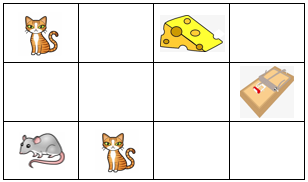
\includegraphics[width=5cm, height=5cm]{pic-toro/exam/cat.png}
    \end{center}
    \begin{enumerate}
        \item ขึ้น ขวา ขวา ขึ้น
        \item ขึ้น ขวา ขวา ขวา
        \item ขึ้น ขึ้น ขวา ขวา
        \item ขึ้น ลง ขวา ขวา
    \end{enumerate}
    \item จากรูปจงเขียนลูกศรนำทางให้เด็กชายไปเอากุญแจเพื่อมาเปิดกล่องสมบัติ
    \begin{center}
        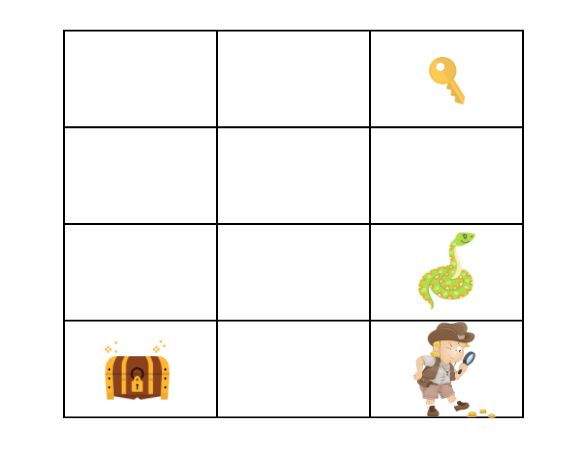
\includegraphics[width=5cm, height=5cm]{pic-toro/exam/treasure.png}
    \end{center}
    \item จากรูปจงเขียนลูกศรนำทางให้เด็กชายไปเอากุญแจเพื่อมาเปิดกล่องสมบัติ
    \begin{center}
        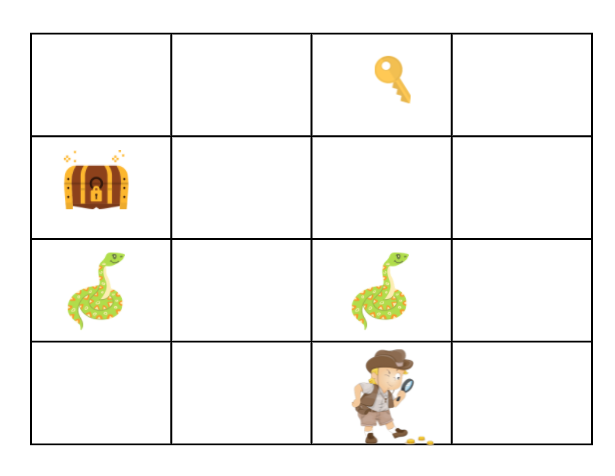
\includegraphics[width=5cm, height=5cm]{pic-toro/exam/treasure2.png}
    \end{center}
    \item นำทางคนป่ากลับถ้ำโดยใช้ลูกศร
    \begin{center}
        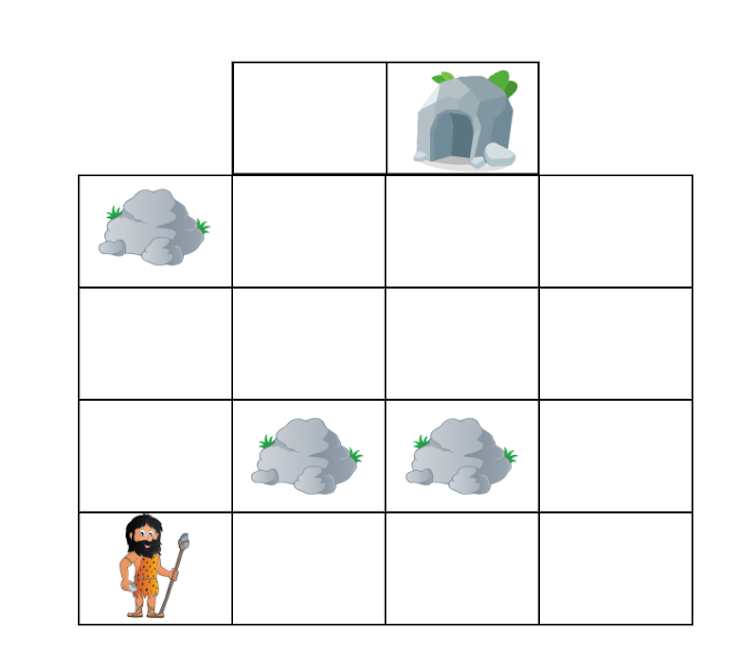
\includegraphics[width=5cm, height=5cm]{pic-toro/exam/cave.png}
    \end{center}
    \clearpage
    \item นำทางหนูไปหาชีสโดยที่ไม่ต้องเจอแมว
    \begin{center}
        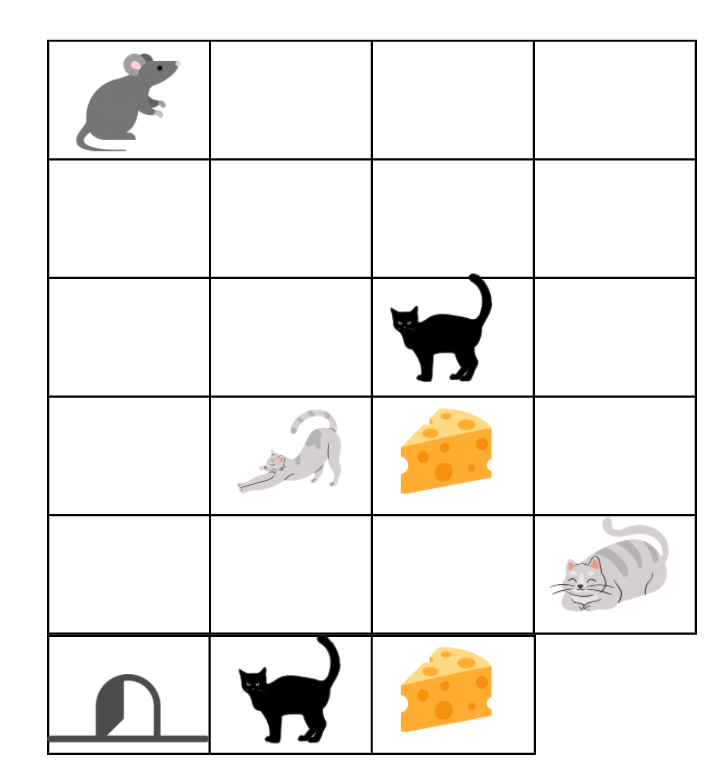
\includegraphics[width=5cm, height=5cm]{pic-toro/exam/cathard.png}
    \end{center}
\end{enumerate}

\section{ตัวอย่าง post-test}
\begin{enumerate}
    \item ข้อใดกล่าวถึงหลักการคิดเชิงคำนวณได้ถูกต้อง
    \begin{enumerate}
        \item เป็นการแก้ปัญหาแบบมีลำดับขั้นตอน
        \item เป็นทักษะที่นักพัฒนาซอฟต์แวร์ต้องมี
        \item เป็นการคิดเหมือนหุ่นยนต์
        \item ข้อ 1 และ ข้อ 2 ถูกต้อง
    \end{enumerate}
    \item จงเรียงลำดับการข้ามถนนบนทางม้าลายที่มีสัญญาณไฟจราจรคนข้ามถนนให้ถูกต้อง
    \begin{itemize}
        \item ไฟจราจรสีเขียว "ข้ามได้"
        \item สังเกตสัญญาณไฟจราจรคนข้ามถนน
        \item เดินข้ามถนนตรงทางม้าลาย
        \item กดปุ่มสัญญาณไฟจราจรคนข้ามถนน
        \item ไฟจราจรสีแดง "หยุดรอ"
    \end{itemize}
    \item กระบวนการแก้ปัญหาจะต้องเริ่มจากขั้นตอนใดเป็นขั้นตอนแรก
    \begin{enumerate}
        \item ดำเนินการแก้ไข
        \item วางแผนการแก้ปัญหา
        \item ตรวจสอบและปรับปรุง
        \item วิเคราะห์และกำหนดรายละเอียดของปัญหา
    \end{enumerate}
    \item ถ้านักเรียนต้องจัดกระเป๋าเพื่อไปเที่ยว ขั้นตอนใดเรียงลำดับได้เหมาะสมที่สุด
    \begin{enumerate}
        \item อาบน้ำ > แต่งตัว > สตาร์ทรถ > เติมน้ำมัน > จัดกระเป๋า
        \item สตาร์ทรถ > เติมน้ำมัน > อาบน้ำ > จัดกระเป๋า > แต่งตัว
        \item อาบน้ำ > แต่งตัว > จัดกระเป๋าอาบน้ำ > สตาร์ทรถ > เติมน้ำมัน
        \item จัดกระเป๋า > อาบน้ำ > แต่งตัว > สตาร์ทรถ > เติมน้ำมัน
    \end{enumerate}
    \item ข้อใดเรียงลำดับการใช้งานคอมพิวเตอร์ได้อย่างเหมาะสมที่สุด
    \begin{enumerate}
        \item เสียบปลั๊ก > กดปุ่มเปิดเครื่อง > กดปุ่มเปิดหน้าจอ > ใช้งาน > กด Shutdown > ปิดหน้าจอ > ถอดปลั๊ก
        \item เสียบปลั๊ก > กดปุ่มเปิดหน้าจอ > ใช้งาน > กด Shutdown > ปิดหน้าจอ > ถอดปลั๊ก
        \item เสียบปลั๊ก > กดปุ่มเปิดเครื่อง > กดปุ่มเปิดหน้าจอ > ใช้งาน > ปิดหน้าจอ > ถอดปลั๊ก
        \item เสียบปลั๊ก > กดปุ่มเปิดหน้าจอ > กดปุ่มเปิดเครื่อง > ใช้งาน > ถอดปลั๊ก > ปิดหน้าจอ
    \end{enumerate}
    \item ช่วยผึ้งหนีหมีและเก็บดอกไม้ไปยังรังผึ้ง
    \begin{center}
        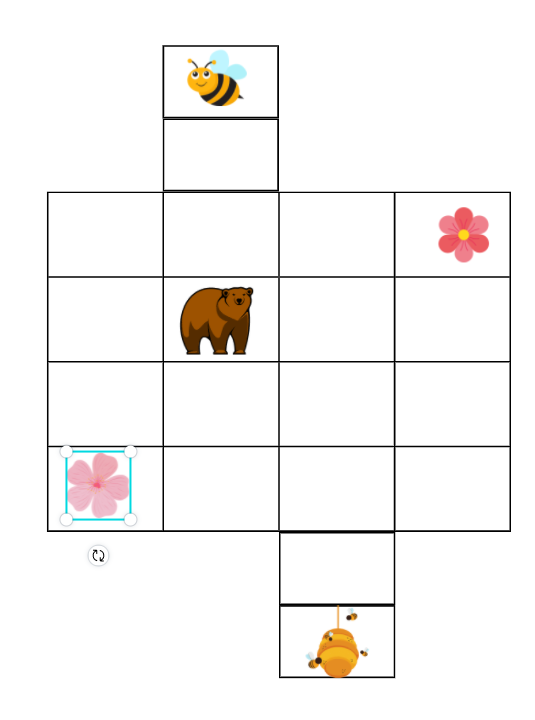
\includegraphics[width=5cm, height=5cm]{pic-toro/exam/bee.png}
    \end{center}
    \item จงลากดินสอไปหาเลข 1 2 3 ตามลำดับแล้วไปยังเส้นชัย
    \begin{center}
        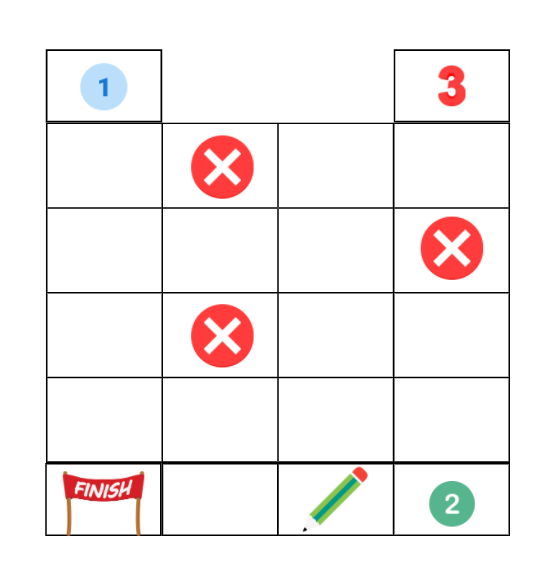
\includegraphics[width=5cm, height=5cm]{pic-toro/exam/pen.png}
    \end{center}
    \item จงรดน้ำต้นไม้ให้ครบทุกต้น
    \begin{center}
        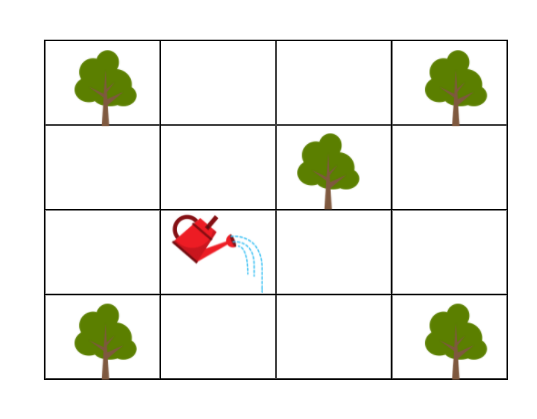
\includegraphics[width=5cm, height=5cm]{pic-toro/exam/treeeasy.png}
    \end{center}
    \item หาวิธีรดน้ำต้นไม้ให้ครบทุกต้นโดยใช้จำนวนครั้งในการเดินน้อยที่สุด
    \begin{center}
        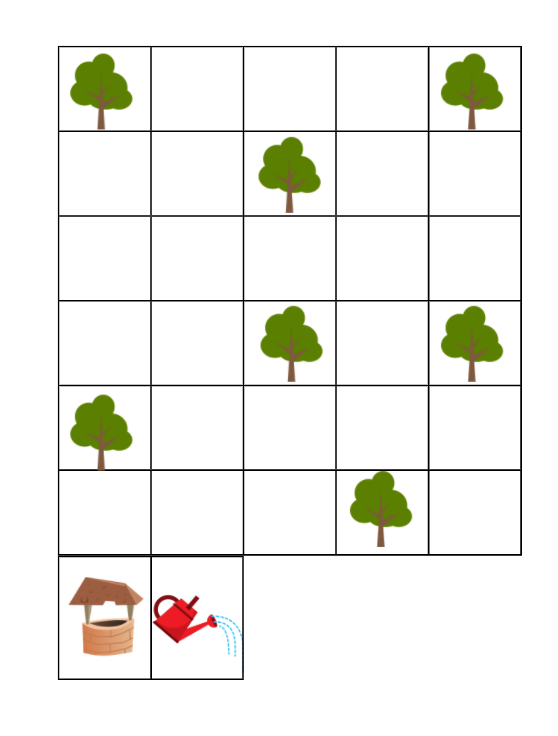
\includegraphics[width=5cm, height=5cm]{pic-toro/exam/treemed.png}
    \end{center}
    \item รดน้ำต้นไม้ให้ครบทุกต้นโดยที่บัวรดน้ำ 1 อันรดน้ำต้นไม้ได้ 3 ครั้ง จากนั้นต้องกลับมาเติมใหม่
    \begin{center}
        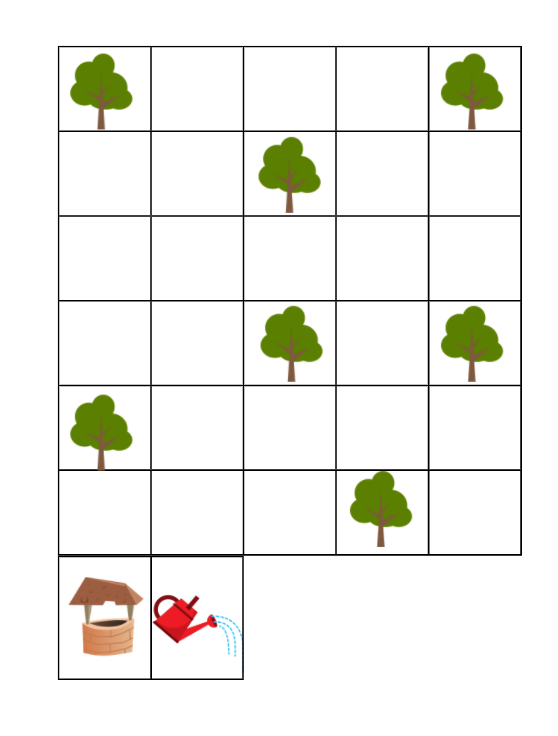
\includegraphics[width=5cm, height=5cm]{pic-toro/exam/treehard.png}
    \end{center} 
\end{enumerate}

\chapter{รายละเอียดและคำอธิบายของแต่ละด่า}
ในภาคผนวกนี้จะประกอบไปด้วยรายละเอียดของแต่ละด่าน ดังนี้
\begin{center}
    \begin{table}[H]
        \begin{center}
            \begin{tabularx}{\textwidth}{|c | X|} 
             \hline
             ด่านที่ & เนื้อหา\\ [0.5ex] 
             \hline\hline
             1 &  ศึกษาวิธีการเล่นเกมโดยให้ตัวละครเดินไป 1 ก้าว \\ 
             \hline
             2 &  ศึกษาวิธีการเปลี่ยนค่าในกล่องคำสั่งโดยให้ตัวละครเดินไป 2 ก้าว \\ 
             \hline
             3 &  ศึกษาวิธีการเปลี่ยนค่าในกล่องคำสั่งโดยให้ตัวละครเดินไป 4 ก้าว \\ 
             \hline
             4 &  ศึกษาคำสั่งใหม่ (หมุน) โดยให้ตัวละครหมุน 1 ครั้งและเดิน 1 ก้าว \\ 
             \hline
             5 &  ศึกษาคำสั่งใหม่ (หมุน) โดยให้ตัวละครหมุน 1 ครั้งและเดิน 4 ก้าว \\ 
             \hline
             6 &  ผสมผสานคำสั่งโดยให้ตัวละครเดินและหมุน \\ 
             \hline
             7 &  ผสมผสานคำสั่งโดยให้ตัวละครเดินและหมุนไปในอีกทิศทาง \\ 
             \hline
             8 &  เพิ่มระดับความยากจากด่านก่อนหน้าโดยต้องใช้คำสั่ง หมุนและเดิน มากขึ้น \\ 
             \hline
             9 &  เพิ่มระดับความยากจากด่านก่อนหน้าโดยต้องใช้คำสั่ง หมุนและเดิน มากขึ้น \\ 
             \hline
             10 &  เพิ่มระดับความยากจากด่านก่อนหน้าโดยต้องใช้คำสั่ง หมุนและเดิน มากขึ้น \\ 
             \hline
             11 &  ศึกษาคำสั่งใหม่ (ทำซ้ำ) โดยให้ผู้ใช้เดินไป 1 ก้าวและครอบด้วยคำสั่งทำซ้ำ \\ 
             \hline
             12 &  ผสมผสานคำสั่ง เดิน, หมุน และทำซ้ำโดยให้ตัวละครเดินเป็นตัว U คว่ำ \\ 
             \hline
             13 &  ผสมผสานคำสั่ง เดิน, หมุน และทำซ้ำโดยให้ตัวละครเดินเป็นซิกเซ็ก \\ 
             \hline
             14 &  ผสมผสานคำสั่ง เดิน, หมุน และทำซ้ำโดยให้ตัวละครเดินเป็นตัว U คว่ำที่ใหญ่กว่า \\ 
             \hline
             15 &  ผสมผสานคำสั่ง เดิน, หมุน และทำซ้ำโดยให้ตัวละครเดินเป็นตัว U คว่ำ โดยมีการหลอก \\ 
             \hline
             16 &  ศึกษาคำสั่งใหม่ (ตัวแปร) \\ 
             \hline
             17 &  ศึกษาวิธีเปลี่ยนค่าของคำสั่งตัวแปร \\ 
             \hline
             18 &  ผสมผสานคำสั่ง เดิน, ตัวแปร และหมุน \\ 
             \hline
             19 &  ผสมผสานคำสั่ง เดิน, ตัวแปร, หมุน และทำซ้ำโดยให้ตัวละครเดินเป็นรูปก้นหอย \\ 
             \hline
             20 &  ผสมผสานคำสั่ง เดิน, ตัวแปร, หมุน และทำซ้ำโดยให้ตัวละครเดินเป็นรูปก้นหอยที่ใหญ่ขึ้น \\ 
             \hline
             21 &  ศึกษาคำสั่งใหม่ (เหยียบบน block สี) โดยให้เดินไปข้างหน้า \\ 
             \hline
             22 &  ผสมผสานคำสั่ง เดิน, หมุน และเหยียบบน block สี \\ 
             \hline
             23 &  ผสมผสานคำสั่ง เดิน, หมุน และเหยียบบน block สีโดยมีการเปลี่ยนค่าของคำสั่ง \\ 
             \hline
             24 &  ผสมผสานคำสั่ง เดิน, หมุน, เหยียบบน block สี และ ทำซ้ำ \\ 
             \hline
             25 &  ผสมผสานคำสั่ง เดิน, หมุน, เหยียบบน block สี และ ทำซ้ำ โดยให้เดินเป็นรูปตัว U คว่ำ \\ 
             \hline
             26 &  เพิ่มจำนวน block สีที่เหยียบได้ โดยในด่านจะมี 2 สี \\ 
             \hline
             27 &  ผสมผสานคำสั่ง เดิน, หมุน, เหยียบบน block สี และ ทำซ้ำ โดยให้เดินเป็นซิกเซ๊ก \\ 
             \hline
             28 &  ผสมผสานคำสั่ง เดิน, หมุน, เหยียบบน block สี และ ทำซ้ำ โดยให้เดินเป็นซิกเซ๊กโดยเพิ่มจำนวนคำสั่งที่ใช้ \\ 
             \hline
             29 &  ผสมผสานคำสั่ง เดิน, หมุน, เหยียบบน block สี และ ทำซ้ำ โดยให้เดินเป็นรูปตัว U คว่ำพร้อมทั้งมีการหลอกการใช้คำสั่ง \\ 
             \hline
             30 &  ผสมผสานคำสั่ง เดิน, หมุน, เหยียบบน block สี และ ทำซ้ำ โดยมี block สีที่เหยียบได้ 3 สี \\ 
             \hline
            \end{tabularx}
        \end{center}
        \caption[ตารางข้อมูลแต่ละด่าน]{ตารางข้อมูลแต่ละด่าน}
        \label{maptable}
    \end{table}
\end{center}

\chapter{\ifcpe คู่มือการใช้งานระบบ\else Manual\fi}

เกมแอปพลิเคชันของโครงงานนี้ จะเป็นเกมแนวอาร์เคดที่สามารถเล่นได้ทุกเพศทุกวัย 
เป็นเกมที่เล่นโดยใช้ทักษะการคิดเชิงคำนวณ เพื่อเล่นให้ผ่านในแต่ละด่าน เก็บคะแนนที่จะได้เป็นดาว แล้วปลดล็อกด่านต่อไปเรื่อยๆ 
โดยภายในเกมจะมีแผนที่อยู่ด้วยกันทั้งหมด 3 แผนที่ แต่ละแผนที่จะมีสภาพแวดล้อมที่แตกต่างกัน และมีด่านอยู่ภายในทั้งหมด 10 
ด่าน แต่ละด่านก็จะมีความยากง่ายแตกต่างกัน โดยจะมีความซับซ้อนและมีเงื่อนไขใหม่ๆ
เพิ่มเข้ามา เพื่อให้ผู้เล่นได้ใช้และพัฒนาทักษะการคิดเชิงคำนวณมากขึ้น

\section{การใช้งานพื้นฐาน}
\begin{enumerate}
    \item หน้าเมนูหลัก กดปุ่ม Start เพื่อไปยังหน้าหน้าเลือกแผนที่ที่ได้ทำการปลดล็อกแล้ว หากต้องการจะกลับมายังหน้าเมนูหลัก ให้กดปุ่ม Home
    \item หน้าเลือกแผนที่ ให้ทำการเลือกแผนที่ที่ต้องการเล่น จากทั้งหมด 3 แผนที่ โดยเริ่มต้นจะปลดล็อกเพียงแผนที่แรกเท่านั้น ผู้เล่นต้องทำการเล่นเก็บดาวเพื่อมาปลดล็อกแผนที่ถัดๆ ไป ดาวที่ผู้เล่นได้รับจะแสดงอยู่มุมขวาบนของหน้าจอ ดังรูปที่ \ref{mapselection}
    \item หน้าเลือกด่านจะประกอบไปด้วยด่านทั้งหมด 10 ด่าน ในแต่ละด่านจะมีดาวให้เก็บ 3 ดาว ระบบจะวัดผลจากคะแนนที่ได้ในด่านนั้นให้เป็นดาว โดยต้องผ่านอย่างน้อย 1 ดาวจึงจะไปยังด่านต่อไปได้
    \item เมื่อผ่านด่านแล้ว จะมีปุ่มให้เลือกกดไปยังด่านถัดไป หากไม่ผ่านด่าน ต้องทำการเล่นอีกครั้งจนกว่าจะได้อย่างน้อย 1 ดาว
\end{enumerate}

\begin{figure}[h!]
    \begin{center}
    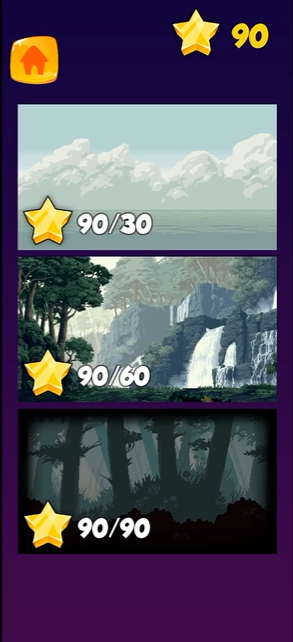
\includegraphics[width=1.75in]{pic/MapSelection.png}
    \end{center}
    \caption[หน้าเลือกแผนที่]{หน้าเลือกแผนที่}
    \label{mapselection}
    \end{figure}

\section{บล็อคคำสั่งทั้งหมดที่ใช้ภายในเกม}
\begin{enumerate}
    \item คำสั่ง move จะทำให้ตัวละครเคลื่อนที่ไปข้างหน้าโดยสามารถกำหนดค่าเป็นตัวเลขได้
    ดังรูปที่~\ref{moveB}
    \item คำสั่ง turn จะทำให้ตัวละครหันหน้าไปในทิศทางที่กำหนดโดนจะมีอยู่ทั้งหมดสองทิศทางให้เลือกคือ ซ้าย หรือ ขวา
    ดังรูปที่~\ref{turnB}
    \item คำสั่ง if จะทำให้ตัวละครทำตามคำสั่งหากเงื่อนไขที่กำหนดนั้นถูกต้อง
    ดังรูปที่~\ref{ifB}
    \item คำสั่ง repeat
    ดังรูปที่~\ref{repeatB}
    \item ชุดคำสั่ง variable ประกอบไปด้วย ตัวแปร 
    ดังรูปที่~\ref{variableB}
\end{enumerate}
\begin{figure}[H]
    \begin{center}
        
\includegraphics[width=2in]{pic/ฺBlockPic/Cmove.png}
    \end{center}
    \caption[คำสั่งเดิน]{คำสั่งเดิน}
    \label{moveB}
\end{figure}
\begin{figure}[H]
    \begin{center}
        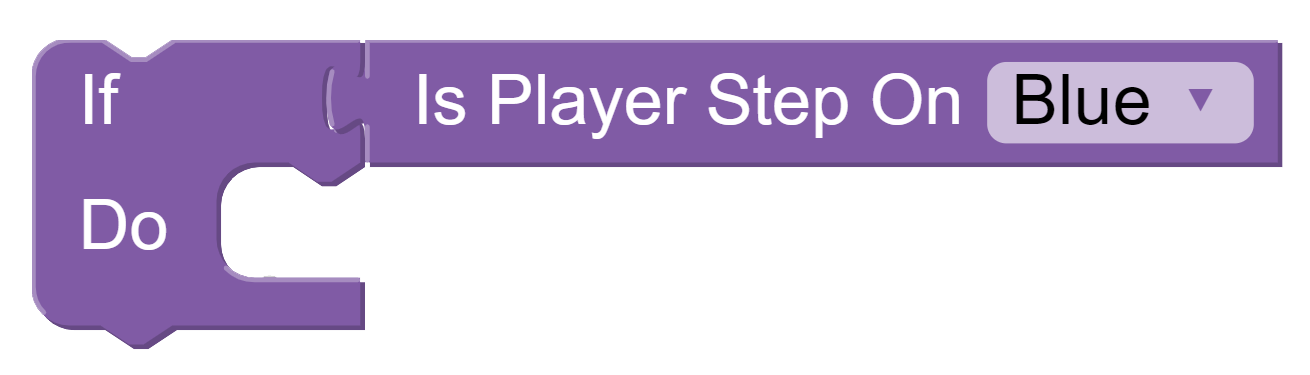
\includegraphics[width=2in]{pic/ฺBlockPic/if.png}
    \end{center}
    \caption[คำสั่งมีเงื่อนไข]{คำสั่งเงื่อนไข}
    \label{ifB}
\end{figure}
\begin{figure}[H]
    \begin{center}
        
\includegraphics[width=2in]{pic/ฺBlockPic/Left.png}
    \end{center}
    \caption[คำสั่งหัน]{คำสั่งหัน}
    \label{turnB}
\end{figure}
\begin{figure}[H]
    \begin{center}
        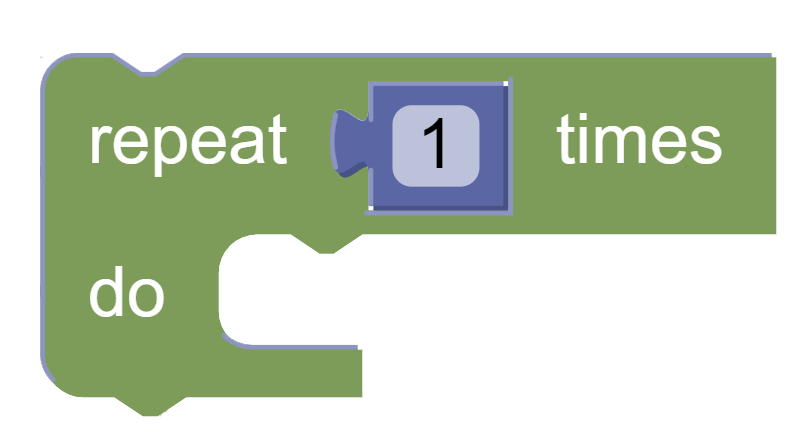
\includegraphics[width=2in]{pic/ฺBlockPic/repeat.png}
    \end{center}
    \caption[คำสั่งทังซ้ำ]{คำสั่งทำซ้ำ}
    \label{repeatB}
\end{figure}
\begin{figure}[H]
    \begin{center}
        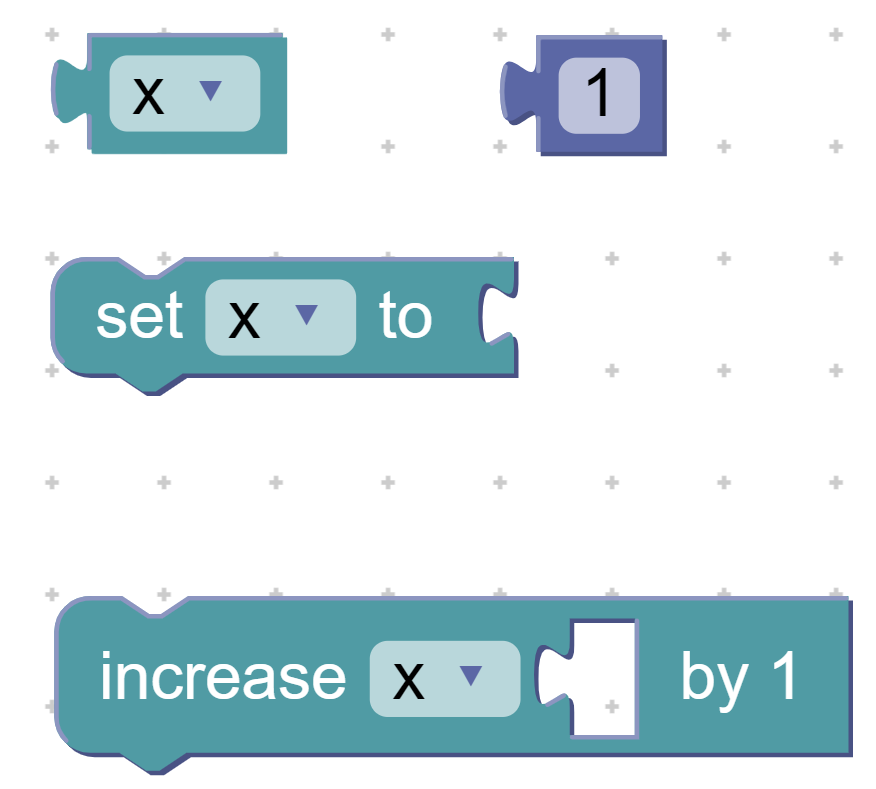
\includegraphics[width=2in]{pic/ฺBlockPic/Variable.png}
    \end{center}
    \caption[ชุดคำสั่งตัวแปร]{ชุดคำสั่งตัวแปร}
    \label{variableB}
\end{figure}

\section{วิธีการเล่น}
\begin{enumerate}
    \item เมื่อเริ่มเกม ตัวละครจะอยู่ห่างจากจุดหมายระยะหนึ่ง ให้นำพาตัวละครไปยังจุดหมายโดยใช้หลักการคิดเชิงคำนวณในวิเคราะห์เส้นทาง 
    
\end{enumerate}

\section{สัญลักษณ์ปุ่มต่างๆภายในเกม}
\begin{enumerate}
    \item ปุ่ม Start กดเพื่อไปยังหน้าเลือกแผนที่
    \item ปุ่ม Home กดเพื่อไปยังหน้าเมนูหลัก
    \item ปุ่มกากบาท กดเพื่อไปยังหน้าเลือกแผนที่
    \item ปุ่ม Start ภายในเกมกดเพื่อทำการเริ่มต้นการทำงานของ Block code
    \item ปุ่ม Reset ภายในเกมกดเพื่อทำการเริ่มต้นวาง Block code ใหม่ทั้งหมด
    \item ปุ่ม Next กดเพื่อทำการไปยังด่านถัดไป
    \item ปุ่ม  Retry กดเพื่อทำการเล่นด่านเดิมอีกครั้ง
    
\end{enumerate}

